% Chapter 1

\chapter{Desarrollo} % Main chapter title

\label{Chapter1} % For referencing the chapter elsewhere, use \ref{Chapter1} 
\label{IntroGeneral}

%----------------------------------------------------------------------------------------

% Define some commands to keep the formatting separated from the content 
\newcommand{\keyword}[1]{\textbf{#1}}
\newcommand{\tabhead}[1]{\textbf{#1}}
\newcommand{\code}[1]{\texttt{#1}}
\newcommand{\file}[1]{\texttt{\bfseries#1}}
\newcommand{\option}[1]{\texttt{\itshape#1}}
\newcommand{\grados}{$^{\circ}$}

%----------------------------------------------------------------------------------------

%\section{Introducción}

%----------------------------------------------------------------------------------------
\section{Introducción}

En el presente trabajo práctico, se desarrolla la implementación de los  algoritmos Monte Carlo ES y Q-Learning en dos modelos que, luego de ser entrenado, son capaces de jugar al tres en linea. El objetivo es poder evaluar la implementación de los algoritmo y compararlos, en sus beneficios y defectos, y en su rendimiento en un juego simple y reducido.

Para lograrlo, se implementaron en lenguaje Python las clases \textit{Board}, y \textit{TicTacToe} que modelan el tablero y las reglas de juego respectivamente (entorno), y la clase abstracta \textit{Player} que da soporte a las operaciones de los posibles jugadores (agentes). Heredando de \textit{Player}, se crearon las clases \textit{UserPlayer}, \textit{BotPlayer},  \textit{MonteCarloEsControl} y \textit{QLearning}  que permiten jugadores humanos, bots aleatorios, modelos guiados por el algoritmo de Monte Carlo ES y modelos guiados por el algoritmo de Q-Learning respectivamente.

Un script principal facilita la ejecución de los casos de uso principales: comenzar un juego entre 2 jugadores o entrenar un modelo utilizando uno de los 2 algoritmos disponibles.

\section{Entorno}

El juego comienza luego de definir 2 tipos de jugadores entre las 3 posibilidades, instanciar la clase \textit{TicTacToe} y ejecutar el método \textit{start}. En ese instante se imprime en pantalla un tablero de tres en línea como se muestra en la figura \ref{fig:board}. 

\begin{figure}[htbp]
	\centering
	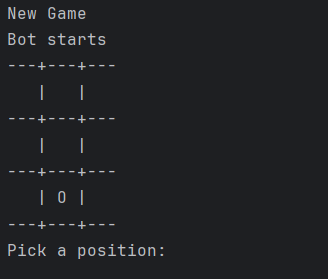
\includegraphics[width=.5\textwidth]{./Figures/board.png}
	\caption{Tablero de tres en linea.}
	\label{fig:board}
\end{figure}

El comportamiento inicial dependerá de los jugadores seleccionados como jugador 1 y 2 y del azar, que le asignará a cualquiera de los anteriores la jugada inicial. Cada vez que un jugador realice una jugada valida, el tablero se refrescará y la partida continuará hasta que haya un ganador o se produzca un empate (tablero lleno). En este momento se detiene el juego y se informa el resultado, como se muestra en la figura \ref{fig:board_end}.

\begin{figure}[htbp]
	\centering
	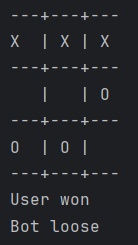
\includegraphics[width=.25\textwidth]{./Figures/board_end.png}
	\caption{Juego finalizado.}
	\label{fig:board_end}
\end{figure}

\section{Agentes}

Cuando  un jugador es humano y le llega su turno, este debe introducir por teclado un número del 0 al 8, correspondientes a las posiciones que se muestran en la figura \ref{fig:human_board}. Si el jugador ingresa una posición inválida o una posición ya tomada, se deberá volver a introducir la jugada.

\begin{figure}[htbp]
	\centering
	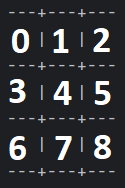
\includegraphics[width=.25\textwidth]{./Figures/human_board.png}
	\caption{Posiciones en el tablero.}
	\label{fig:human_board}
\end{figure}

El bot aleatorio elige, en forma automática y aleatoria, cualquier posición disponible en el tablero. Este no sigue ninguna estrategia y resulta útil únicamente para probar el juego y para realizar el entrenamiento de los modelos disponibles.

Los agentes con modelos entrenables realizan movimientos en forma automática siguiendo una política aprendida. En cada turno observan el estado actual del tablero, y toman la acción que se evaluó como mejor opción para ese estado durante el entrenamiento.

\section{Entrenamiento}

\subsection{Monte Carlo ES}

Para entrenar el agente de Monte Carlo ES, se ejecutaron múltiples juegos consecutivos de tres en línea donde participaban el agente en entrenamiento y bots aleatorios. Dentro del agente de Monte Carlo ES se implementó el algoritmo de la figura \ref{fig:algorithm_monte_carlo}, con los siguientes detalles:
\begin{itemize}
    \item \(A(s)\) contiene las acciones posibles, que son jugar las posiciones del 0 al 8.
    \item S contiene los estados posibles del tablero. El tablero de tres en línea tiene en total \(3^9 = 19.683\) estados diferentes, la mayoría de los cuales son ilegales.
    \item  Dado que resulta costoso generar las políticas iniciales aleatorias para todos los estados del tablero y también filtrar solo los estados posibles (alrededor de 5.478), se decidió comenzar con \(\pi(s)\) y \(Q(s,a)\) vacíos e inicializarlos en forma aleatoria a medida que el agente se encontraba con estados que nunca había visto antes.
    \item Para el comienzo exploratorio de Monte Carlo, se ejecutaron en el tablero un número aleatorio de jugadas aleatorias alternadas entre jugador 1 y 2 previo a comenzar el episodio. Cabe destacar que se realizó un chequeo del estado del tablero luego de estas inicializaciones para verificar la validez.
    \item Como recompensa se asignó -0.1 por cada jugada que no concluyera en el final del juego, -10 a una jugada perdedora, -2 a una jugada de empate y 10 a una jugada ganadora.
    \item Adicionalmente se limito el número de jugadas del agente en 20 y se agrego una penalización de -50 si se supera este valor. De esta forma se prioriza aprender a jugar posiciones válidas.
    \item Se fijo un factor de descuento de 0.9.
    \item El entrenamiento se repitió durante 500.000 episodios, demorando aproximadamente una hora.
    \item Los valores anteriores se obtuvieron en forma empírica, a partir de varios entrenamientos y analizando los resultados obtenidos.
\end{itemize} 

\begin{figure}[htbp]
	\centering
	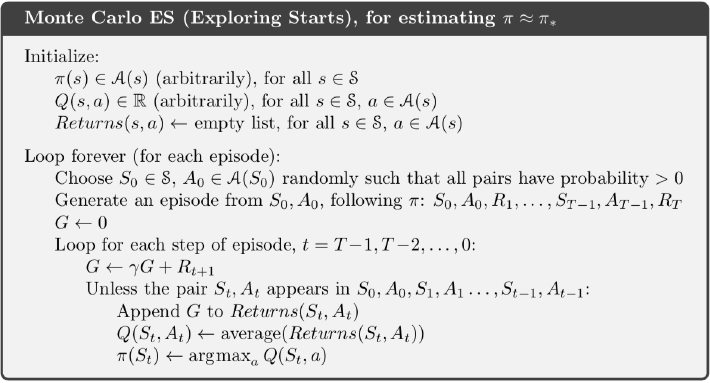
\includegraphics[width=0.8\textwidth]{./Figures/algorithm_monte_carlo.png}
	\caption{Algoritmo de Mote Carlo ES.}
	\label{fig:algorithm_monte_carlo}
\end{figure}

\subsection{Q-Learning}

Para entrenar el agente de Q-Learning, se ejecutaron múltiples juegos consecutivos de tres en línea donde participaban el agente en entrenamiento y bots aleatorios. Dentro del agente de Q-Learning se implementó el algoritmo de la figura \ref{fig:algorithm_q_learning}, con los siguientes detalles:
\begin{itemize}
    \item \(A(s)\) contiene las acciones posibles y S contiene los estados posibles del tablero, al igual que en el caso anterior.
    \item  Q-Learning no necesita inicio aleatorio del estado del ambiente, por lo que los diferentes episodios de juego empezaron con el tablero vacío.
    \item Las recompensas se mantuvieron como en el caso anterior: -0.1 por cada jugada que no concluyera en el final del juego, -10 a una jugada perdedora, -2 a una jugada de empate, 10 a una jugada ganadora y -50 por superar las 20 jugadas.
    \item Se fijo un \(\alpha\) (tasa de aprendizaje) de 0.1, un \(\gamma\) (factor de descuento) de 0.9 y un \(\epsilon\) (factor de exploración) de 0.2.
    \item El entrenamiento se repitió durante 500.000 episodios, demorando aproximadamente 5 minutos.
\end{itemize} 

\begin{figure}[htbp]
	\centering
	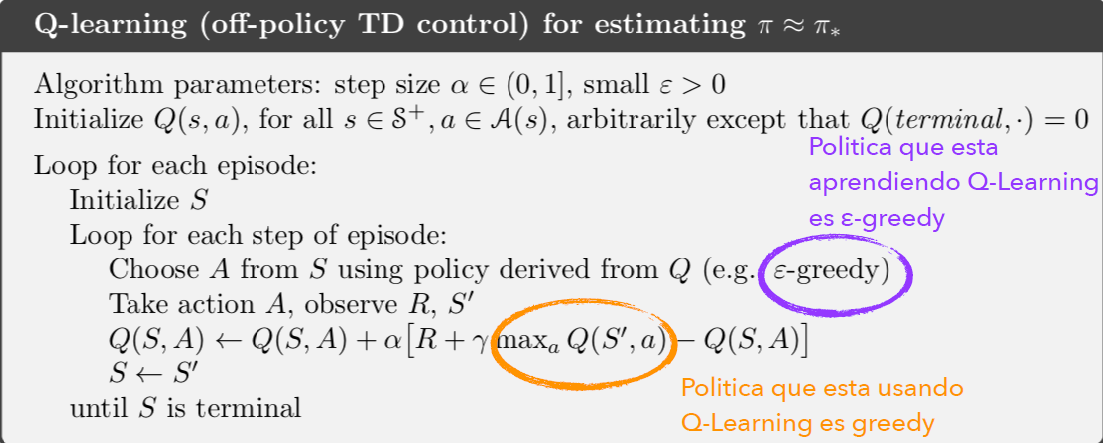
\includegraphics[width=0.8\textwidth]{./Figures/algorithm_q_learning.png}
	\caption{Algoritmo de Q-Learning.}
	\label{fig:algorithm_q_learning}
\end{figure}

\section{Resultados}

\subsection{Monte Carlo ES}

Luego de entrenar el agente Monte Carlo ES se obtuvo la curva de recompensa de la figura \ref{fig:monte_carlo_episode_rewards}  y la curva de éxito (juegos ganados) de la figura \ref{fig:monte_carlo_success_rate}.

En la figura \ref{fig:monte_carlo_episode_rewards} se observa que la media de la recompensa aumenta lentamente con el paso de los episodios desde un valor de 0 hasta aproximadamente 5, lo que nos indica que el modelo está entrenándose correctamente. También, observamos en la figura \ref{fig:monte_carlo_success_rate} que el modelo alcanza un porcentaje de juegos ganados de aproximadamente 0.7, es decir, el modelo gana el 70\% de las partidas contra un bot aleatorio, por lo que su política es mejor que elegir posiciones al azar.

\clearpage

\begin{figure}[htbp]
	\centering
	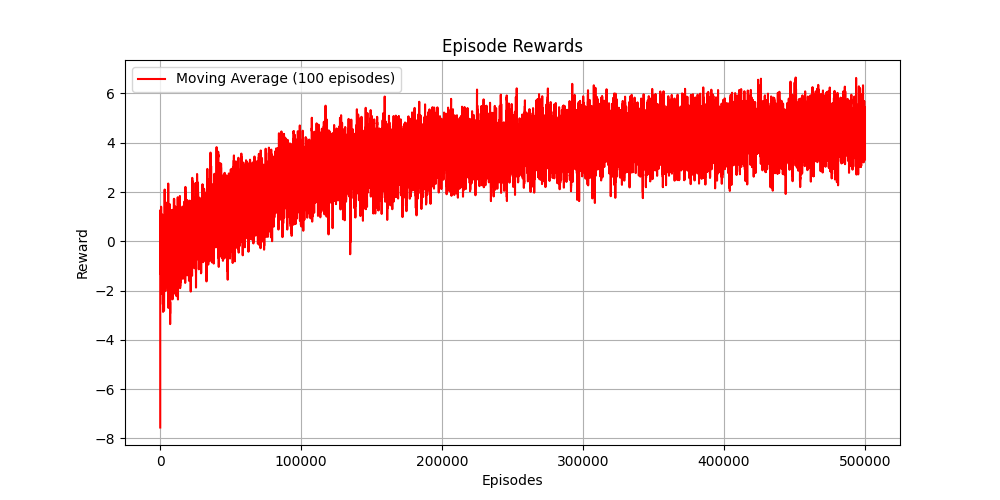
\includegraphics[width=\textwidth]{./Figures/monte_carlo_episode_rewards.png}
	\caption{Recompensa por episodio para algoritmo de Monte Carlo ES, suavizado con una media móvil de 100 episodios.}
	\label{fig:monte_carlo_episode_rewards}
\end{figure}

\begin{figure}[htbp]
	\centering
	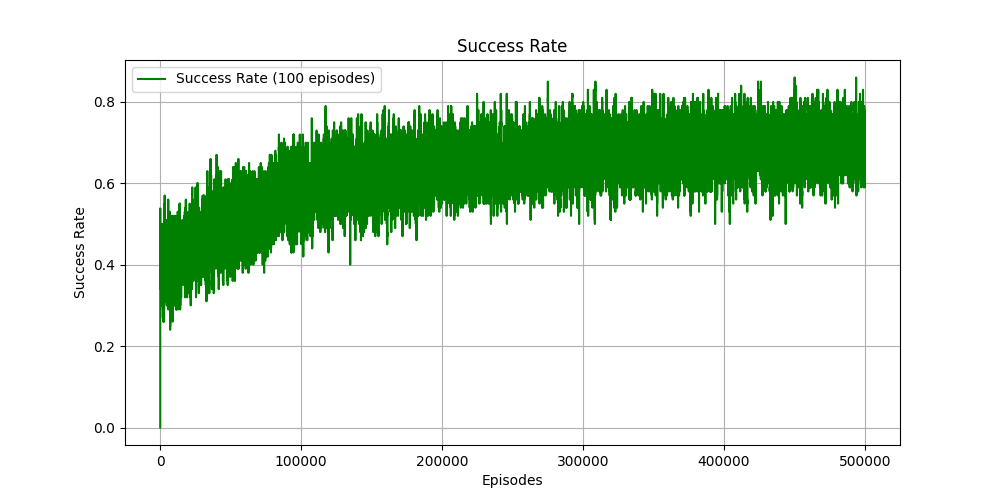
\includegraphics[width=\textwidth]{./Figures/monte_carlo_success_rate.png}
	\caption{Curva de éxito (porcentaje de juegos ganados en los últimos 100 episodios) para algoritmo de Monte Carlo ES.}
	\label{fig:monte_carlo_success_rate}
\end{figure}

Al jugar en contra del modelo, se observa que se obtuvo un modelo capaz de identificar las estrategias principales del tres en línea. Por ejemplo, si el modelo comienza el juego, este toma siempre el centro del tablero como se observa en la figura \ref{fig:monte_carlo_center}. También, si tiene posibilidad de ganar, toma la posición ganadora; o por el contrario, si el contrincante tiene posibilidad de ganar, intenta bloquear esa posibilidad, como se observa en las figuras \ref{fig:monte_carlo_win} y \ref{fig:monte_carlo_block}.

\clearpage

\begin{figure}[htbp]
	\centering
	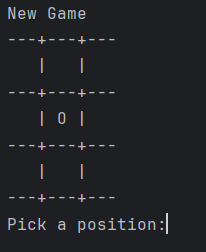
\includegraphics[width=0.25\textwidth]{./Figures/monte_carlo_center.png}
	\caption{Agente tomando el centro.}
	\label{fig:monte_carlo_center}
\end{figure}

\begin{figure}[htbp]
	\centering
	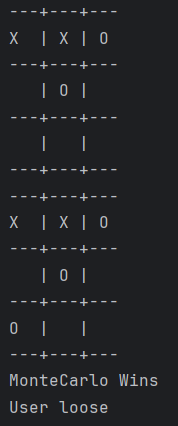
\includegraphics[width=0.25\textwidth]{./Figures/monte_carlo_win.png}
	\caption{Agente tomando la posición ganadora.}
	\label{fig:monte_carlo_win}
\end{figure}

\begin{figure}[hbt!]
	\centering
	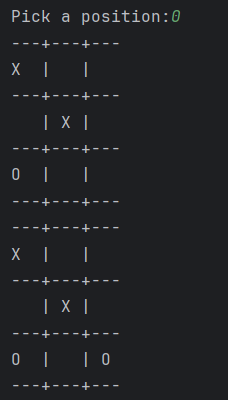
\includegraphics[width=0.25\textwidth]{./Figures/monte_carlo_block.png}
	\caption{Agente bloqueando la posición ganadora del humano.}
	\label{fig:monte_carlo_block}
\end{figure}

Lo sorprendente es que el modelo también aprende estrategias avanzadas, Por ejemplo, si teniendo tomado el centro el usuario elige posición 1, 3, 5 o 7, la victoria esta asegurada con el patrón de la figura \ref{fig:monte_carlo_advanced}. A la vez, si el jugador humano intenta ejecutar la misma estrategia, el agente de Monte Carlo ES la evita eligiendo las esquinas como su primer movimiento.

\begin{figure}[htbp]
	\centering
	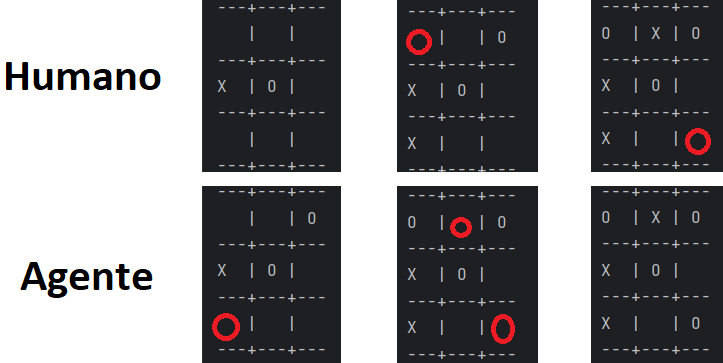
\includegraphics[width=\textwidth]{./Figures/monte_carlo_advanced.png}
	\caption{Agente ejecutando estrategia que asegura la victoria. En rojo posiciones ganadoras.}
	\label{fig:monte_carlo_advanced}
\end{figure}

Como contrapartida el agente no es perfecto, cuando se intenta ejecutar sobre el mismo otra estrategia ganadora mostrada en la figura \ref{fig:monte_carlo_exception}, este falla eligiendo repetidamente una posición ya tomada. Esto se debe a que en el entrenamiento no se exploró el espacio de estados y acciones lo suficiente como para encontrar una mejor política.

\begin{figure}[htbp]
	\centering
	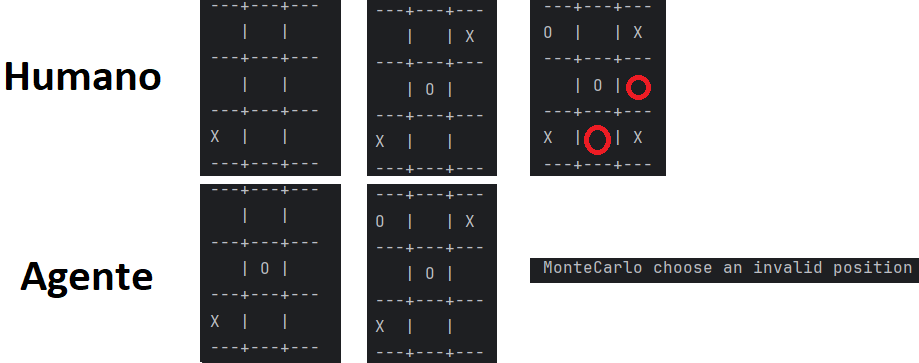
\includegraphics[width=\textwidth]{./Figures/monte_carlo_exception.png}
	\caption{Agente fallando en tomar posiciones válidas.}
	\label{fig:monte_carlo_exception}
\end{figure}

\subsection{Q-Learning}

Luego de entrenar el agente Q-Learning se obtuvo la curva de recompensa de la figura \ref{fig:q_learning_episode_rewards}  y la curva de éxito de la figura \ref{fig:q_learning_success_rate}.

\clearpage

\begin{figure}[htbp]
	\centering
	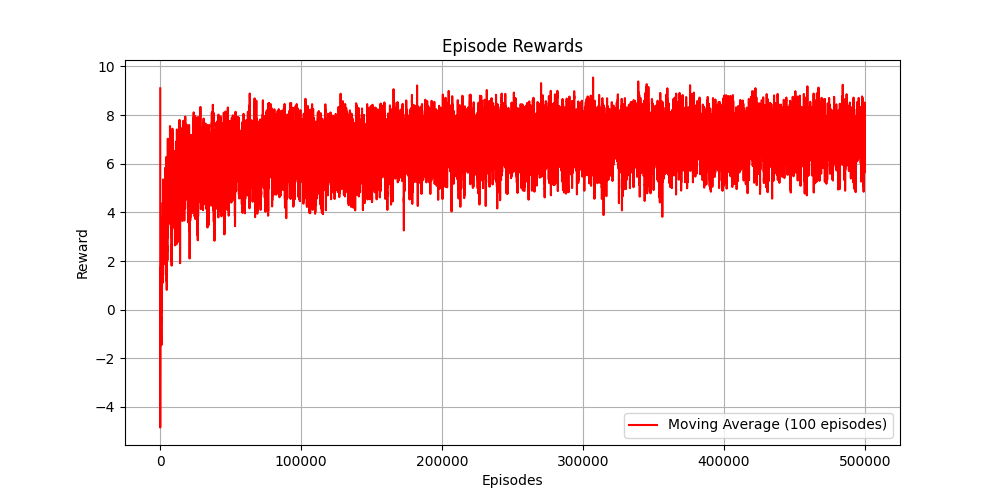
\includegraphics[width=\textwidth]{./Figures/q_learning_episode_rewards.png}
	\caption{Recompensa por episodio para algoritmo de Q-Learning, suavizado con una media móvil de 100 episodios.}
	\label{fig:q_learning_episode_rewards}
\end{figure}

\begin{figure}[htbp]
	\centering
	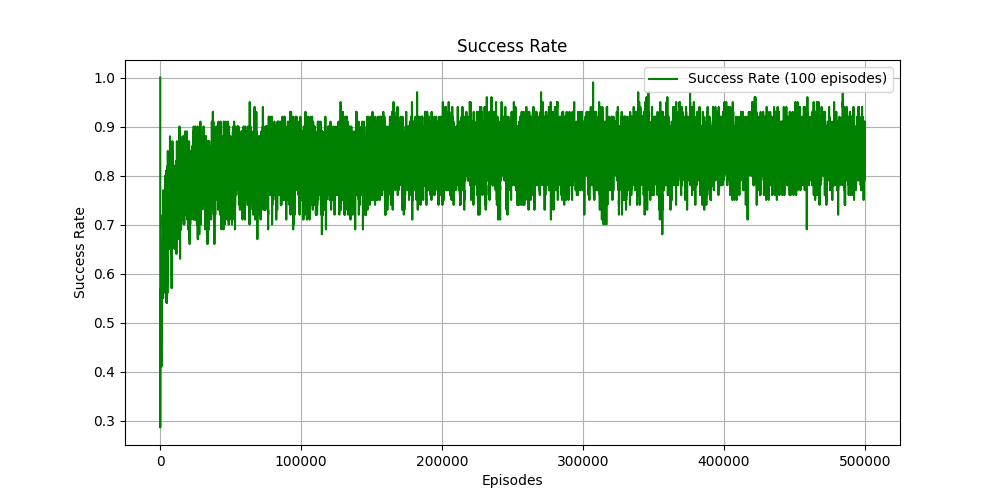
\includegraphics[width=\textwidth]{./Figures/q_learning_success_rate.png}
	\caption{Curva de éxito (porcentaje de juegos ganados en los últimos 100 episodios) para algoritmo de Q-Learning.}
	\label{fig:q_learning_success_rate}
\end{figure}

En primer lugar se observa que el entrenamiento también converge y rápidamente, con solo 100.000 episodios el modelo ya estaría entrenado. Luego se observa que los valores de recompensa y de tasa de éxito alcanzados son mayores respecto al modelo anterior, aunque esto no es indicativo de mayor calidad ya que Monte Carlo ES requiere de inicios aleatorios que pueden llevar a estados que terminan siempre en jugadas perdedoras o empate.

Al jugar en contra del modelo, se obtienen los mismos resultados que en el modelo anterior, se observa que se aprenden estrategias básicas y también avanzadas. A diferencia del anterior, el modelo de Q-Learning parece ser mas consistente en sus resultados, teniendo menos situaciones donde elige posiciones ya tomadas.

\section{Conclusiones}

Ambos algoritmos mostraron resultados muy buenos en el desafío planteado, no solamente aprendiendo los movimientos básicos, sino también aprendiendo estrategias avanzadas lo cual fue inesperado. 

Comparando, Q-Learning mostró un mejor desempeño con una convergencia en menor cantidad de episodios de entrenamiento, gracias a su aprendizaje off-policy y al algoritmo de exploración \(\epsilon\)-greedy. Monte Carlo ES, al aprender solo en base a la política ejecutada y requerir de comienzos aleatorios para la exploración demora una mayor cantidad de episodios en explorar todos los pares estado-acción posibles. Más aún, los comienzos exploratorios de Monte Carlo ES agregan complejidad a la implementación, ya que requiere de código adicional que permita fijar el ambiente en un estado inicial determinado. 

Como puntos débiles de ambos algoritmos, aún en un juego simple como el tres en línea, se deben mantener estructuras (como la tabla Q) para todos los estados posibles del tablero, que en este caso es del orden de los miles, lo que implica un costo computacional moderado. Otro punto débil de ambos algoritmos es que no pueden ``extrapolar`` conocimiento, es decir aprovechar lo aprendido para un estado para resolver estados similares, que en este caso sería una cualidad deseable ya que el tres en línea es un juego simétrico si se rota el tablero.

\section{Trabajo futuro}

Como trabajo futuro se plantea enfrentar ambos algoritmos en un entrenamiento a la par, para observar el comportamiento. Lo esperable sería que el modelo de Q-Learning comience ganando el mayor porcentaje de partidas y que, luego de muchos episodios, la mayoría de las partidas terminen en empate.
